\chapter{Geometric Problems Related to Muon Physics at Daya Bay}\label{app:a}
The Daya Bay neutrino experiment is equipped with excellent muon tracker detectors, thus more aspects of the muon physics can be studied by reconstructing muon tracks. Since in each collision the muon deflection is usually small, the muon track is usually approximated by a straight line. Besides, detectors usually are of regular shapes such as being spherical or cylindrical, they can by modeled by simple 3D algebraic equations. There are several interesting questions concerning to the relations between different geometric objects and in this appendix simple solutions to these pure analytic geometry problems are presented.

\section{Track Length in a Cylinder}
At Daya Bay the deposited energy of each muon is registered. Since the ionization energy loss is roughly proportional to the track length the muon traverses, track length is also a quantity of interest. Because the energy registered by the detector is mainly from the scintillation light when the muon passes the scintillator region, we are interested in the track length contained in the outer acrylic vessel where liquid scintillator resides. Besides, neutrons are detected mainly by the Gd capture and Gd is only present inside the inner acrylic vessel. When measuring the neutron production per unit length, the track length inside the IAV is also needed. Here we want to solve the problem that given a cylinder centered at the origin and a straight line passing through it, find the length of the line inside the cylinder.

\paragraph{Problem:}Given a cylinder with radius $r$ and height $2r$ and a straight line intersecting with the cylinder which passes a point $\vec{p}$ with a normalized direction vector $\hat{v}$, find the length of the line segment contained in the cylinder.

\paragraph{Solution:}
One way to solve this problem is to write down the equations for the the cylinder and the straight line in some convenient coordinate system and solve for the intersection points. However when implementing this method in computer codes, the idea is obscured by the lines of code to solve the simultaneous algebraic equations. Another more coordinate free and clearer to implement method is stated below.

First we deal with the intersection problem of the straight line with an infinitely long cylinder. After the intersection points are found, the top and bottom planes are restored, and the intersection points are adjusted if necessary. The axis of the cylinder is also a straight line and together with the track line form two skew lines. The closest distance $d$ between the skew lines can be used to identify whether the track line intersects the cylinder and is easily found. Suppose the points where the closest distance happens are $\vec{q}_c$ on the cylinder axis and $\vec{q}$ on the track line. $\vec{q}_c$ and $\vec{q}$ satisfy the equations
\begin{eqnarray}
	\vec{q}_c&=&\vec{p}_c+t_c\hat{v}_c \\
	\vec{q}&=&\vec{p}+t\hat{v}
\end{eqnarray}
where $\vec{p}_c$, $\hat{v}_c$ are the point and the direction vector of the cylinder axis and $t_c$ and $t$ are the parameters to be determined. Since the line formed by the two closest points is perpendicular to both of the skew lines, the vector $\vec{q}-\vec{q}_c$ is parallel to the cross product of the direction vectors of the skew lines,
\begin{equation}\label{closest_app_orig}
	\vec{q}-\vec{q}_c=\vec{p}-\vec{p}_c+t\hat{v}-t_c\hat{v}_c=k\hat{v}\times\hat{v}_c
\end{equation}
Let $\vec{p}_r=\vec{p}-\vec{p}_c$ and $\vec{n}=\hat{v}\times\hat{v}_c$, Equation~\ref{closest_app_orig} becomes
\begin{equation}\label{closest_app}
	\vec{p}_r+t\hat{v}-t_c\hat{v}_c=k\vec{n}
\end{equation}
Dot Equation~\ref{closest_app} with $\vec{n}$ on both sides and note that $\vec{n}\cdot \hat{v}=\vec{n}\cdot \hat{v}_c=0$, we have
\begin{equation}
	kn^2=\vec{p}_r\cdot \vec{n}
\end{equation}
Therefore the closest distance $d$ is given by
\begin{equation}
	d=\abs{\vec{q}-\vec{q}_c}=\abs{kn}=\frac{\abs{\vec{p}_r\cdot \vec{n}}}{n}=\frac{\abs{(\vec{p}-\vec{p}_c)\cdot (\hat{v}\times\hat{v}_c)}}{\abs{\hat{v}\times\hat{v}_c}}
\end{equation}
Note that if $d>r$ then the track line will never intersect the cylinder and there is no solution to this problem.

To find the parameters $t$ and $t_c$, first form the cross product of both sides of Equation~\ref{closest_app} with $\vec{n}$
\begin{equation}\label{par_eq}
	\vec{p}_r\times \vec{n}+t\hat{v}\times \vec{n}-t_c\hat{v}_c\times \vec{n}=0
\end{equation}
Now to get $t$, dot both sides of Equation~\ref{par_eq} with $\vec{v}_c$ and note that $\vec{v}_c\cdot (\vec{v}_c\times \vec{n})=0$ and $\vec{v}_c\cdot (\vec{v}\times \vec{n})=(\vec{v}_c\times \vec{v})\cdot \vec{n}=-n^2$. Then we get
\begin{equation}
	t=\vec{v}_c\cdot (\vec{p}_r\times \vec{n})/n^2
\end{equation}
Similarly we can dot Equation~\ref{par_eq} with $\vec{v}$ to obtain $t_c$.

Now that we have the shortest distance between the skew lines and the corresponding points, we are ready to solve for the intersection points. Figure~\ref{fig:cyl_line} shows a cylinder in blue and a straight line in red passing through it. $\overleftrightarrow{CD}$ is the cylinder axis and $\overleftrightarrow{Q_iQ_o}$ is the track line. Given the closest points $O$, $Q$, and angle $\angle QQ_iB=\angle QQ_oA=\theta$, we want to find $\ell=\overline{QQ_i}=\overline{QQ_o}$.
\begin{figure}
	\centering
	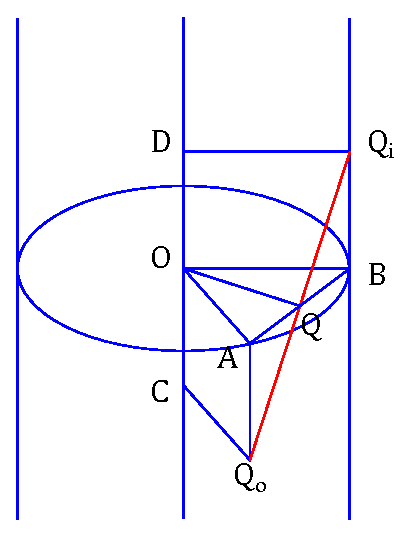
\includegraphics[width=.4\textwidth]{figures/appendixA/cylinder_line.eps}
	\caption{An illustration of a cylinder and a straight line passing through it. Given points $O$ and $Q$, we want to find $Q_i$ and $Q_o$.}
	\label{fig:cyl_line}
\end{figure}

$\ell$ can actually be found by simple arguments. First we start from $Q_i$ and draw a straight line on the cylinder surface parallel to the cylinder axis. This line will intersect with the circle centered at $O$. We call the point $B$. Similarly we can find point $A$ starting with point $Q_o$. Since $\overline{OA}=\overline{OB}=r$, the radius of the cylinder, $\triangle OAB$ is isoceles. By symmetry, $\triangle OQA$ is congruent to $\triangle OQB$, and therefore $\overline{OQ}$ is perpendicular to $\overline{AB}$. Meanwhile, $\triangle QBQ_i$ and $\triangle QAQ_o$ are also right triangles. From $\triangle OQB$ and $\triangle QBQ_i$ we have the relation
\begin{gather}
  \overline{QB}^2=\ell^2\sin^2\theta=\overline{OB}^2-\overline{OQ}^2 \\
  \Rightarrow \ell=\frac{\sqrt{r^2-d^2}}{\sin\theta}
\end{gather}
Once $\ell$ is known, $Q_i$ and $Q_o$ are also known.

The last step is to restore the top and bottom planes of the cylinder and rescale the solution points if necessary. In order to simply the notation, here we adopt the coordinate system with the origin at the cylinder center and the $z$ axis parallel to the cylinder axis. In this coordinate system the top cylinder plane has the equation $z=z_t$ and bottom plane has the equation $z=z_b$. Suppose in this coordinate system $Q_i$ has coordinate $Q_i(q_{ix},q_{iy},q_{iz})$. There are three conditions concerning to the ordering of $q_{iz}$, $z_t$ and $z_b$:
\begin{enumerate}
	\item $q_{iz}<z_b$. There is no solution to this problem.
	\item $z_b<q_{iz}<z_t$. $Q_i$ is the right answer and nothing has to be done.
	\item $z_t<q_{iz}$. $Q_i$ has to be moved along the track line until it touches the top plane. The new point is
	\begin{equation}
		\vec{q'}_i=\vec{q}-\frac{z_t-q_z}{q_{iz}-q_z}\hat{v}
	\end{equation}
	where $Q$ has the coordinate $Q(q_x,q_y,q_z)$ and $\hat{v}$ has a direction with $v_z<0$.
\end{enumerate}

We do a similar check on the point $Q_o$. If there is a solution, the track length is $\overline{Q_iQ_o}$.

Now we look at the problem of finding a cylindrical fiducial volume with an arbitrary axis inside a bigger cylinder so that it has the maximum length and is completely inscribed in the bigger cylinder.

\paragraph{Problem:} Given a cylinder with radius $R$ and height $2R$, a straight line with a point $p_0$ and a normalized direction $\hat{v}$, find a cylinder with the straight line as its axis and a fixed radius $r<R$ such that the cylinder has a maximum  length and is completely inside the given cylinder.

\paragraph{Solution:} We use the coordinate system centered at the center of the given cylinder with $z$ axis parallel to the cylinder axis. Again we start with two infinitely long cylinders, one with radius $R$ and the other with radius $r<R$. If they do intersect, the intersection is a curve. First we want to find, at least numerically, the coordinates of the points in the curve.
\begin{figure}
	\centering
	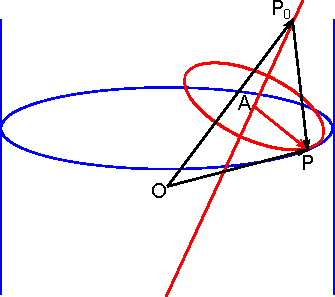
\includegraphics[width=.5\textwidth]{figures/appendixA/inscribe.pdf}
	\caption{A point $P$ belonging to the surface of the big and small cylinders simultaneously.}
	\label{fig:inscribe}
\end{figure}
Figure~\ref{fig:inscribe} shows a point $P$ belonging to the given and the fiducial cylinders simultaneously. Since $P$ is on the fiducial cylinder, from Pythagorean theorem we have
\begin{equation}\label{eq:pytha}
	\overline{AP_0}^2+\overline{AP}^2=\overline{PP_0}^2
\end{equation}
Now $\overline{AP_0}=r$, $\overline{AP}=|(\vec{p}-\vec{p}_0)\cdot \hat{v}|$, $\overline{PP_0}=|\vec{p}-\vec{p}_0|$. Because $P$ also belongs to the given cylinder, it has coordinate $P(R\cos\phi,R\sin\phi,z)$. Suppose $\vec{p}-\vec{p}_0=(X,Y,Z)$ and $\hat{v}=(v_x,v_y,v_z)$, by substituting the coordinates and numbers into Equation~\ref{eq:pytha} we obtain
\begin{equation}
	(1-v_z^2)Z-2v_z(v_xX+v_yY)Z+[X^2+Y^2-(v_xX+v_yY)^2-r^2]=0
\end{equation}
where
\begin{eqnarray}
	X &=& R\cos\phi-p_{0x} \\
	Y &=& R\sin\phi-p_{0y} \\
	Z &=& z-p_{0z}
\end{eqnarray}
For each value of $\phi$ there is a corresponding quadratic equation. Practically we can scan for $\phi$ with some small step, solve the equation for $z$, and find the coordinates of the points in the common curve. Usually there are $\phi$ values with two real roots and $\phi$ values without any real root. This is due to the topology of the intersection curve. We plot the $z$ versus $\phi$ plot. If there is solution to this problem, there are two closed curve in this plot. If there are less then two curves, there is no solution. Figure~\ref{fig:no_solution_cylinders} and Figure~\ref{fig:with_solution_cylinders} show examples without and with solution. From the figures we clearly see that the problem has a solution only if there are two closed curves.
\begin{figure}
	\centering
  \subfloat[$z$ vs. $\phi$]{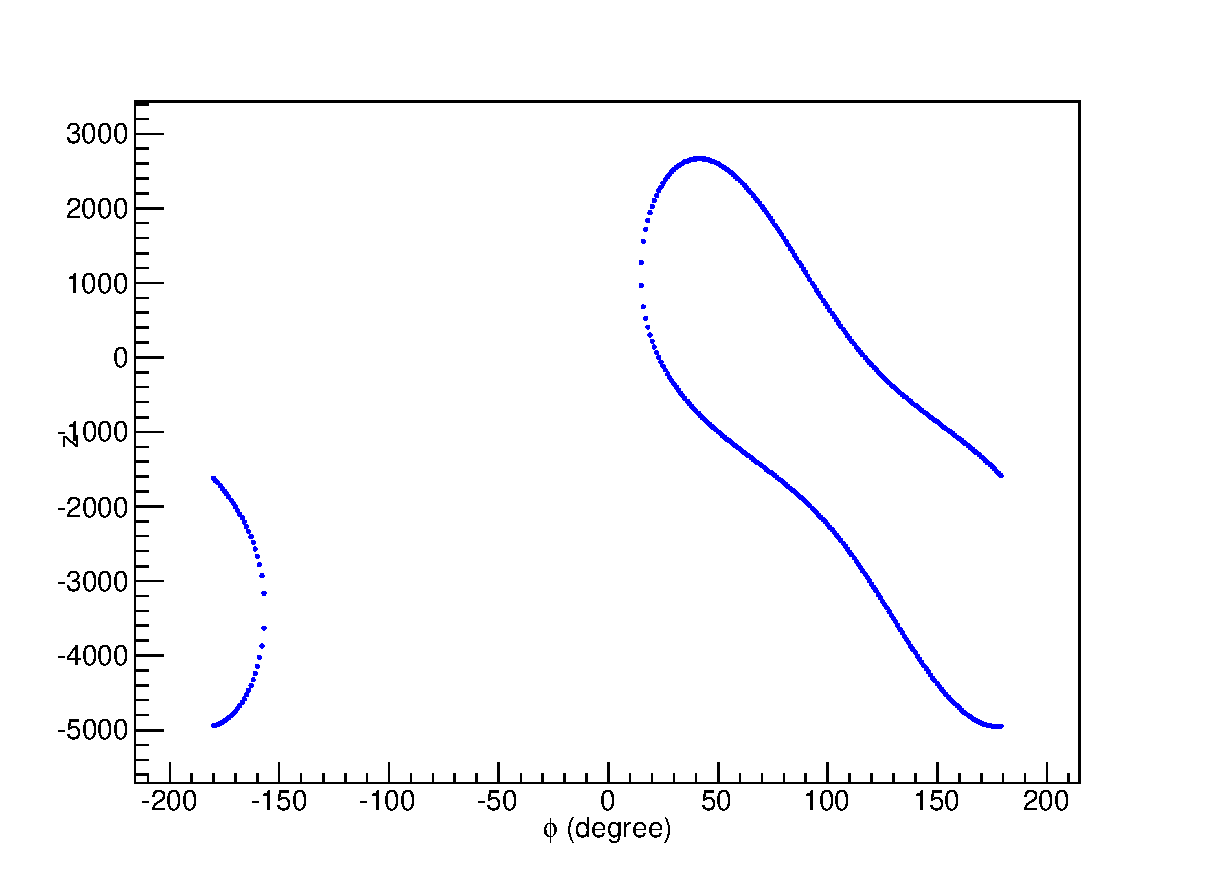
\includegraphics[height=.25\textheight]{figures/appendixA/curve1.eps}}
  \qquad
	\subfloat[3D Model]{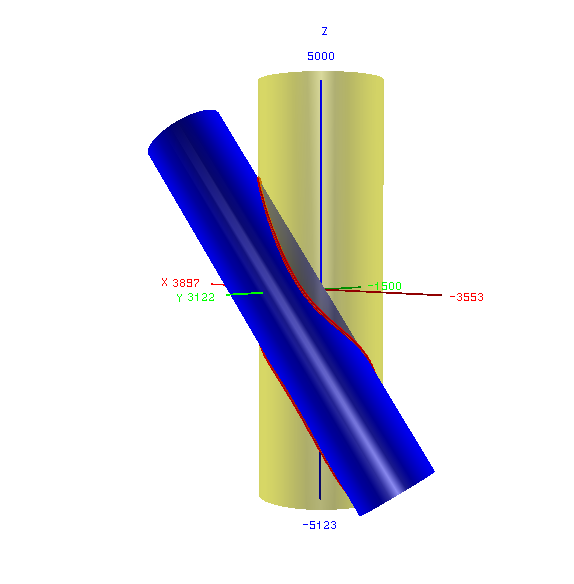
\includegraphics[height=.25\textheight]{figures/appendixA/cyl1.png}}
	\caption{The $z-\phi$ plot and the 3D model of an example without solution.}
	\label{fig:no_solution_cylinders}
\end{figure}
\begin{figure}
	\centering
  \subfloat[$z$ vs. $\phi$]{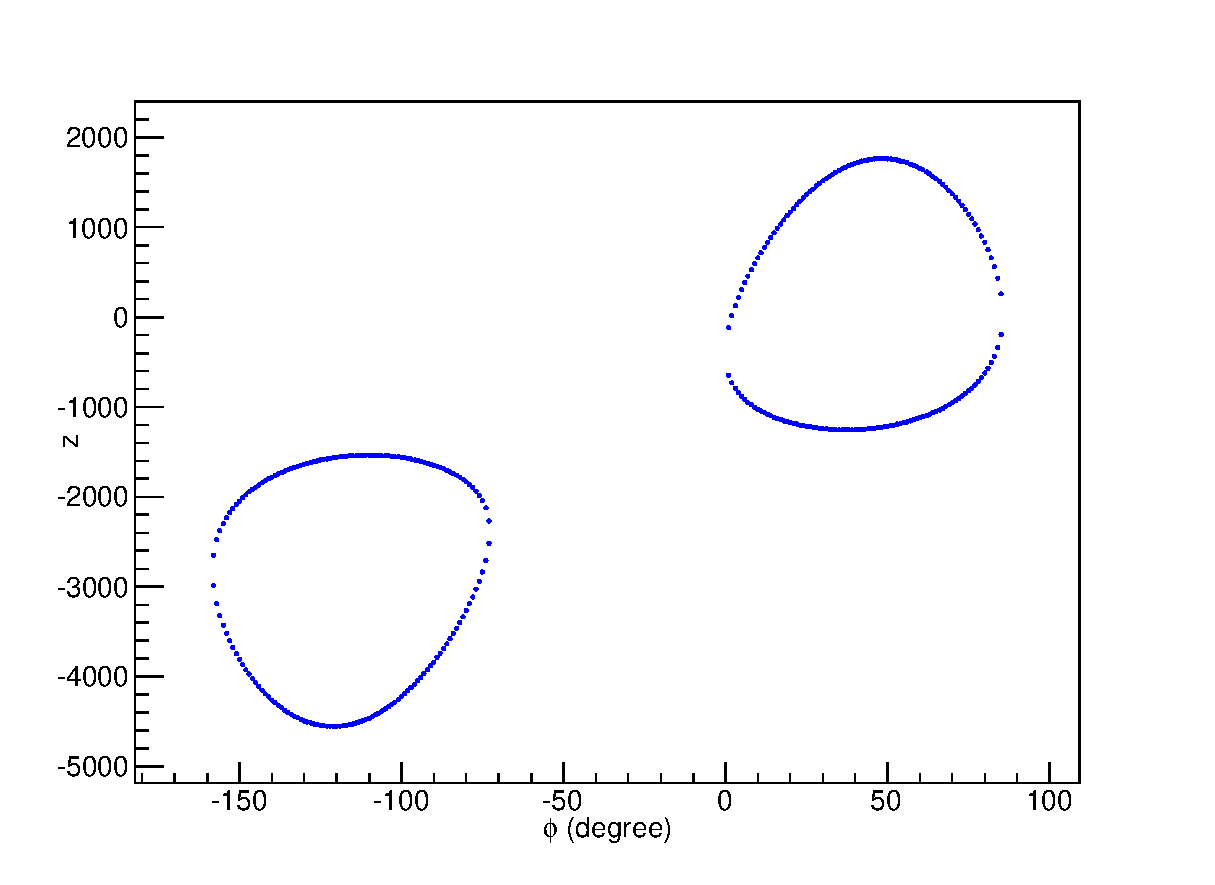
\includegraphics[height=.25\textheight]{figures/appendixA/curve2.eps}}
  \qquad
	\subfloat[3D Model]{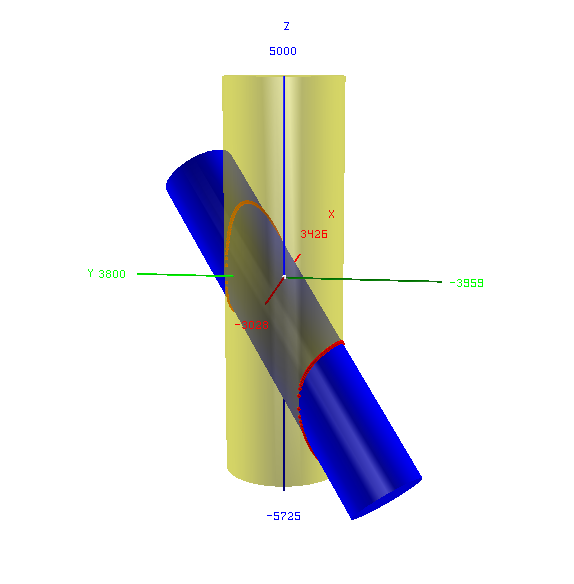
\includegraphics[height=.25\textheight]{figures/appendixA/cyl2.png}}
	\caption{The $z-\phi$ plot and the 3D model of an example with solution.}
	\label{fig:with_solution_cylinders}
\end{figure}
Here we also introduce a convenient track coordinate, with origin at the point of the track line $p_0$ and a $t$ axis along the track's direction vector $\hat{v}$. For each point in each closed curve we can calculate the $t$-value by projection,
\begin{equation}
	t=\left(\vec{p}-\vec{p}_0\right)\cdot \hat{v}
\end{equation}
Now we look for the four numbers,
\begin{eqnarray}
	t^{(i)}_M&=&\sup\left\{ t^{(i)}|\vec{p}^{(i)}\in C^{(i)}\right\} \\
	t^{(i)}_m&=&\inf\left\{ t^{(i)}|\vec{p}^{(i)}\in C^{(i)}\right\}
\end{eqnarray}
where $i=1,2$ for the two closed curves $C^{(i)}$, sort the four numbers, take the middle two numbers and call the larger one $t_{bot}$ and the smaller one $t_{top}$. Then we arrive at two candidate planes. Each one has $\hat{v}$ as its normal vector and passes $\vec{p}_{bot}=\vec{p}_0+t_{bot}\hat{v}$ and $\vec{p}_{top}=\vec{p}_0+t_{top}\hat{v}$, respectively.

Now we restore the top and bottom planes of the detector cylinder. If the top circle of the track cylinder protrudes the top plane of the detector cylinder, slide it along the track until it just touches the top plane of the detector cylinder. The same applies to the bottom circle of the track cylinder.